% LaTeX Article Template
\documentclass{article}
\usepackage{amssymb, amsmath, amsfonts, amsthm, latexsym}
\usepackage{graphicx}
\newcommand{\C}{\mathbb {C}}
\newcommand\tab[1][1cm]{\hspace*{#1}}
\newcommand\smalltab[1][0.3cm]{\hspace*{#1}}

\begin{document}

\begin{center}
\textbf{CSCI 362 Deliverable 2: SugarLabs}
\end{center}


\begin{center}

{The Chocolate L'Eclercs}\\
\vspace{0.2cm}
{Alex Skiff, Blaine Billings, Carson Barber}\\
{Chase Myers, Justin Willis}\\
\vspace{0.2cm}

\end{center}

\section{Deliverable 2: Introductory Test Plan}
\subsection{Testing Process}
We have divided the process of our test plan for our five introductory test cases into the evaluation of three main subsystems. They are described as follows:
\begin{enumerate}
\itemsep-0.5em
\item \textbf{Profile}: The \textbf{profile} subsystem of SugarLabs includes all files relevant to the creation of a user's profile, including the age, gender, etc. This will be evaluated based on input/ouput matching as well as on exception handling for invalid input.
\item \textbf{Journal}: The \textbf{journal} subsystem of SugarLabs includes all files relevant for the upkeep of a user's journal. Much like with the first subsystem, this will be evaluated based on input/output matching as well as on exception handling for invalid input.
\item \textbf{Activity}: The \textbf{activity} subsystem of SugarLabs includes all files relevant to tracking a user profile's assigned activities, essentially providing running assessment list for the user. This will be evaluated based on correctness of logged information with regards to simulated performed actions.
\end{enumerate}
\subsection{Requirements Traceability}
\label{ReqTrace}
For the aforementioned subsystems, the following files will be evaluated. This information is included for the ease of tracking the testing process and the evaluated files as well as the understanding of what processes in specific are being investigated.
\begin{enumerate}
\itemsep-0.5em
\item \textbf{Profile}: colorpicker.py, agepicker.py, genderpicker.py for color, age, and gender selection, respectively, in the user profile creation process.
\item \textbf{Journal}: journalactivity.py, journalentrybundle.py, journalwindow.py for activity logging, entry bundling, and graphical output, respectively, in the user journal editing and viewing.
\item \textbf{Activity}: buddy.py for the activity assignment in the user activity view.
\end{enumerate}
\subsection{Tested Items}
In this section, we described the specifc items mentioned in Section \ref{ReqTrace} and give an in-depth description of how they are to be tested through our framework. Figure \ref{Figure2} shows a visualization of three three general susbsystems and their associated test cases.
\begin{figure}
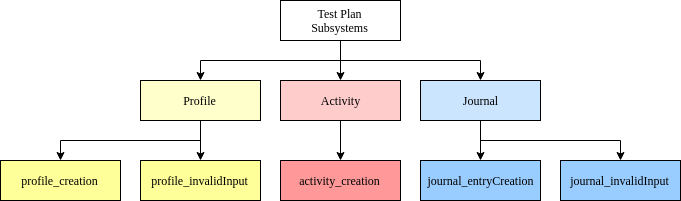
\includegraphics[scale=0.5]{../imgs/Figure2.png}
\caption{Overview of test plan subsystems and their associated test cases. (made using draw.io)}
\label{Figure2}
\end{figure}
\subsubsection{Profile}
The testing of this subsystem and the respective colorpicker.py, agepicker.py, and genderpicker.py files will begin with the creation of a test\textunderscore profile.py program with specific test\textunderscore profile\textunderscore creation and test\textunderscore profile\textunderscore invalidInput functions as test cases. These test cases go as follows:
\begin{enumerate}
\itemsep-0.5em
\item \textbf{test\textunderscore profile\textunderscore creation}: This function will consist of the selection of a valid color and a gender and the input of a valid age. The test will be passed if profile creation is carried through with according input and without the throwing of an exception.
\item \textbf{test\textunderscore profile\textunderscore invalidInput}: This function will consist of the input of an invalid color, gender, or age. The test will be passed if profile creation with this input throws an exception.
\end{enumerate}
\subsubsection{Journal}
The testing of this subsystem and the respective journalactivity.py, journalentry-bundle.py, and journalwindow.py files will begin with the creation of a test\textunderscore journal.py program with specific test\textunderscore journal\textunderscore entryCreation and test\textunderscore journal\textunderscore invalidInput functions as test cases. These test cases go as follows:
\begin{enumerate}
\itemsep-0.5em
\item \textbf{test\textunderscore journal\textunderscore entryCreation}: This function will consist of the opening of the journal entry window followed by the inputting of a valid journal entry name. The test will be passed if profile creation is carried through with according input and without the throwing of an exception.
\item \textbf{test\textunderscore journal\textunderscore invalidInput}: This function will consist of the opening of the journal entry window followed by the inputting of an invalid journal entry name (special characters, escaped characters, etc.). The test will be passed if profile creation with this input throws an exception.
\end{enumerate}
\subsubsection{Activity}
The testing of this subsystem and the respective buddy.py file will begin with the creation of a test\textunderscore activity.py program with specific test\textunderscore activity\textunderscore creation function as a test case. These test case goes as follows:
\begin{enumerate}
\itemsep-0.5em
\item \textbf{test\textunderscore activity\textunderscore creation}: This function will consist of the opening of the creation of a new activity and its assignment to a specific user profile. The test will be passed if activity creation is carried through with according input, assigned to the relevant profile, and without the throwing of an exception.
\end{enumerate}
\subsection{Testing Schedule}
The tentative schedule for our testing plan has been defined as follows:
\begin{itemize}
\itemsep-0.5em
\item[] \textbf{11/9/2018}: Completion of automated testing framework
\item[] \textbf{11/19/2018}: Completion of design and implementation of testing framework; Evaluation of twenty-five test cases
\item[] \textbf{11/28/2018}: Completion of code injection of 5 faults; Testing of chosen twenty-five test cases with faulty code.
\end{itemize}
\subsection{Test Recording Procedures}
Each of the implemented test cases will be coded in python and run through the terminal as described in the first deliverable. For easy auditing and understanding of previous tests, this code will include the date, time, and current software version with all output automatically being written to a log file for that specific date. These will be aggregated in a \textbf{testing} folder in the root directory of this testing framework's project.
\subsection{Hardware and Software Requirements}
As of the time of this document being written, Sugar Labs requires the local operating system to be either Debian 0.110 or higher, Fedora, or Ubuntu 16.04 or higher. In addition, Python 2.7, the main codebase of the software, must be installed alongside the sugar-artwork, sugar-datastore, and sugar-toolkit-gtk3 packages which can all be obtained directly from the terminal. For building the project, the packages intltool, libglib2.0-dev, and gtk+-3.0 should also be installed on the system. 
\subsection{Constraints}
Though there are not many constraints limiting the testing process of this project, we must plan to be punctual in every step of our testing framework's implementation as required by the general outline of this course. Due to the nature of this project (in it being carried out in an educational setting), we need not worry about budgeting, staff, or weekly meeting presentations, all of which are often necessitated in government or industry settings.
\subsection{System Tests}
The system tests will primarily consist of checking relevant software installations. The following software, shown with their according verification commands, will be used to check that the system is up-to-date and able to run SugarLabs:
\begin{itemize}
\itemsep-0.5em
\item \textbf{Python}: python -v
\item \textbf{intltool}: intltool -\--help
\item \textbf{autoconf}: autconf -h
\item \textbf{libglib2.0-dev}: dpkg -\--get-selections $\mid$ grep libglib2.0-dev
\item \textbf{gtk+-3.0}: dpkg -\--get-selections $\mid$ gtk-3.0
\end{itemize}

\end{document}